\subsection{Supervised Model Evaluation}
\label{sec:modelres}

TODO

\subsubsection{Hyperparameter Tuning}

TODO

\begin{figure}[h]
	\centering
	\begin{subfigure}[b]{0.5\textwidth}
		\centering
		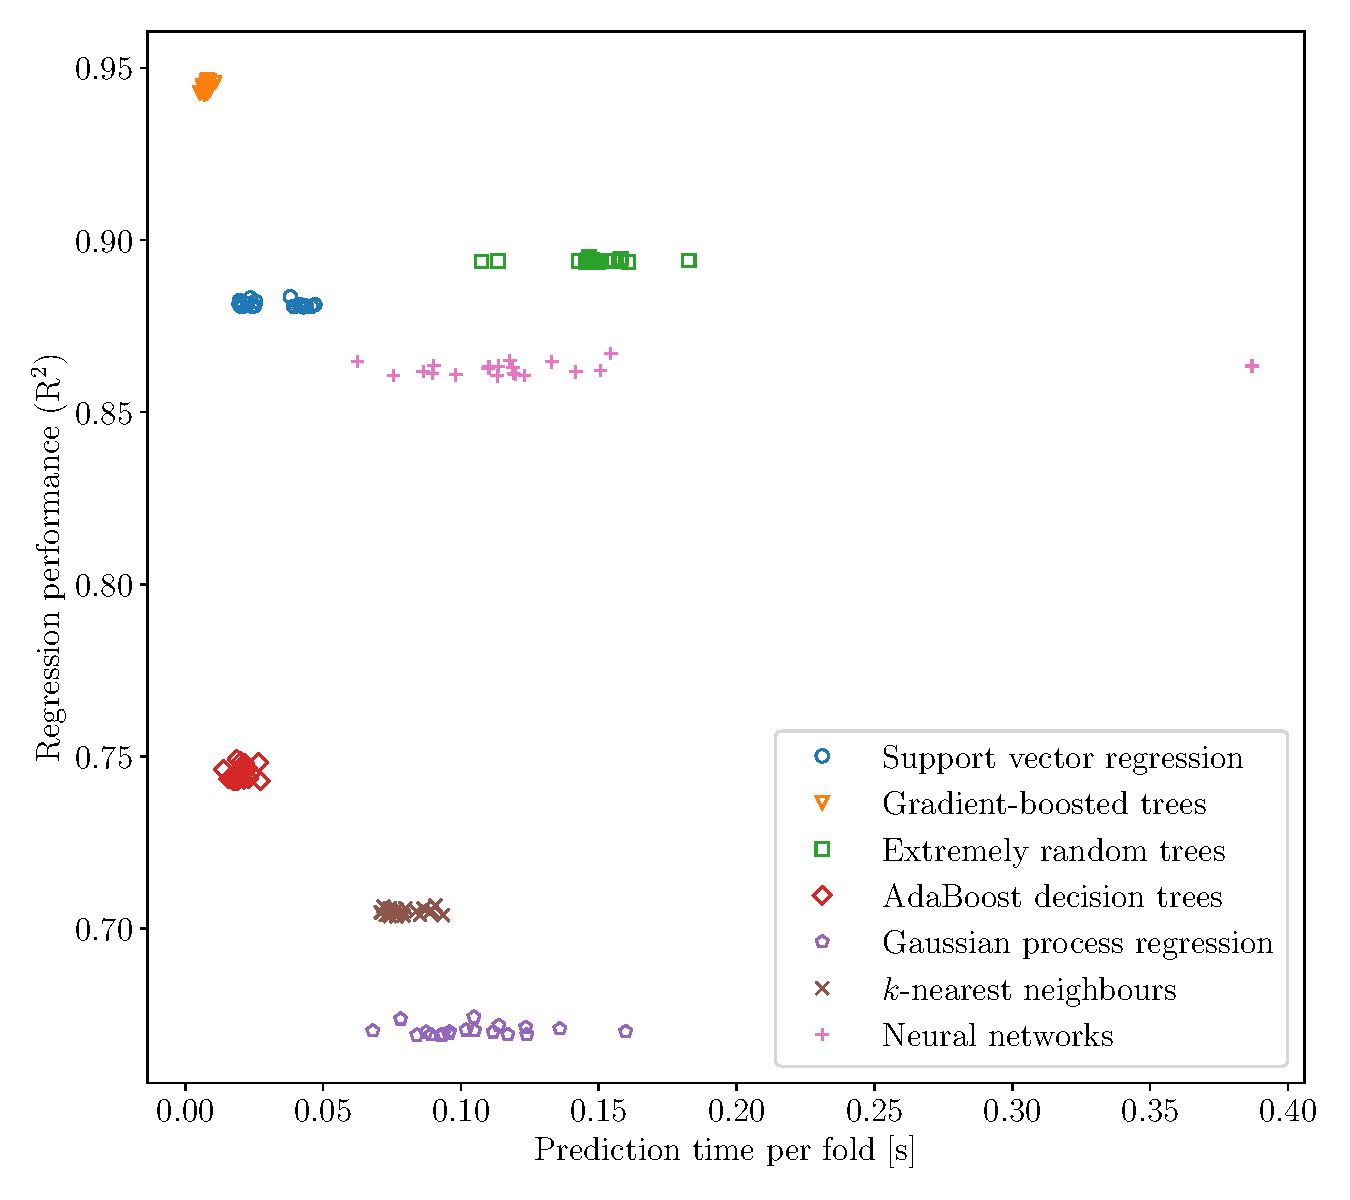
\includegraphics[width=\linewidth]{exp1_time_vs_reg}
		% TODO: only a placeholder, regenerate when data becomes available
		\caption{Experiment 1 (single slice)}
	\end{subfigure}\hfill%
	\begin{subfigure}[b]{0.5\textwidth}
		\centering
		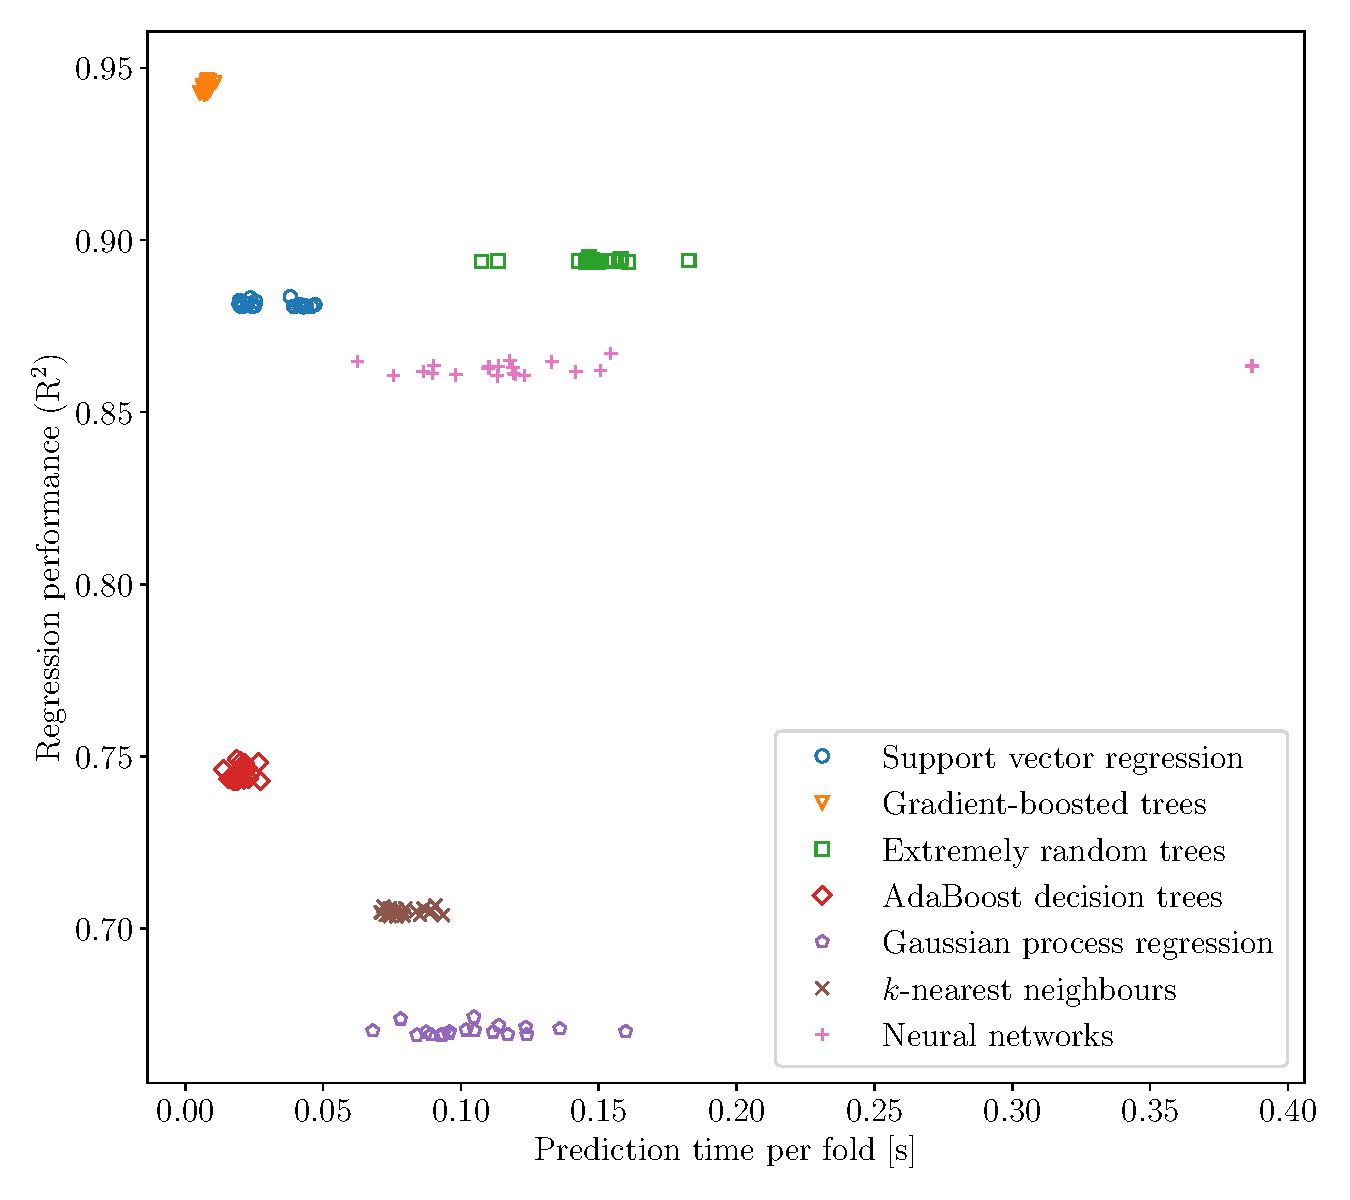
\includegraphics[width=\linewidth]{exp1_time_vs_reg}
		% TODO: only a placeholder, regenerate when data becomes available
		\caption{Experiment 2 (full dataset)}
	\end{subfigure}
	\caption{Regression performance (as $R^2$) plotted against mean
	prediction time for the best $N$~models of each surrogate class.} % TODO. fill N
	\label{fig:time-vs-reg}
\end{figure}


\subsubsection{Scaling Benchmark}

TODO

\begin{figure}[h]
	\centering
	\begin{subfigure}[b]{0.333\textwidth}
		\centering
		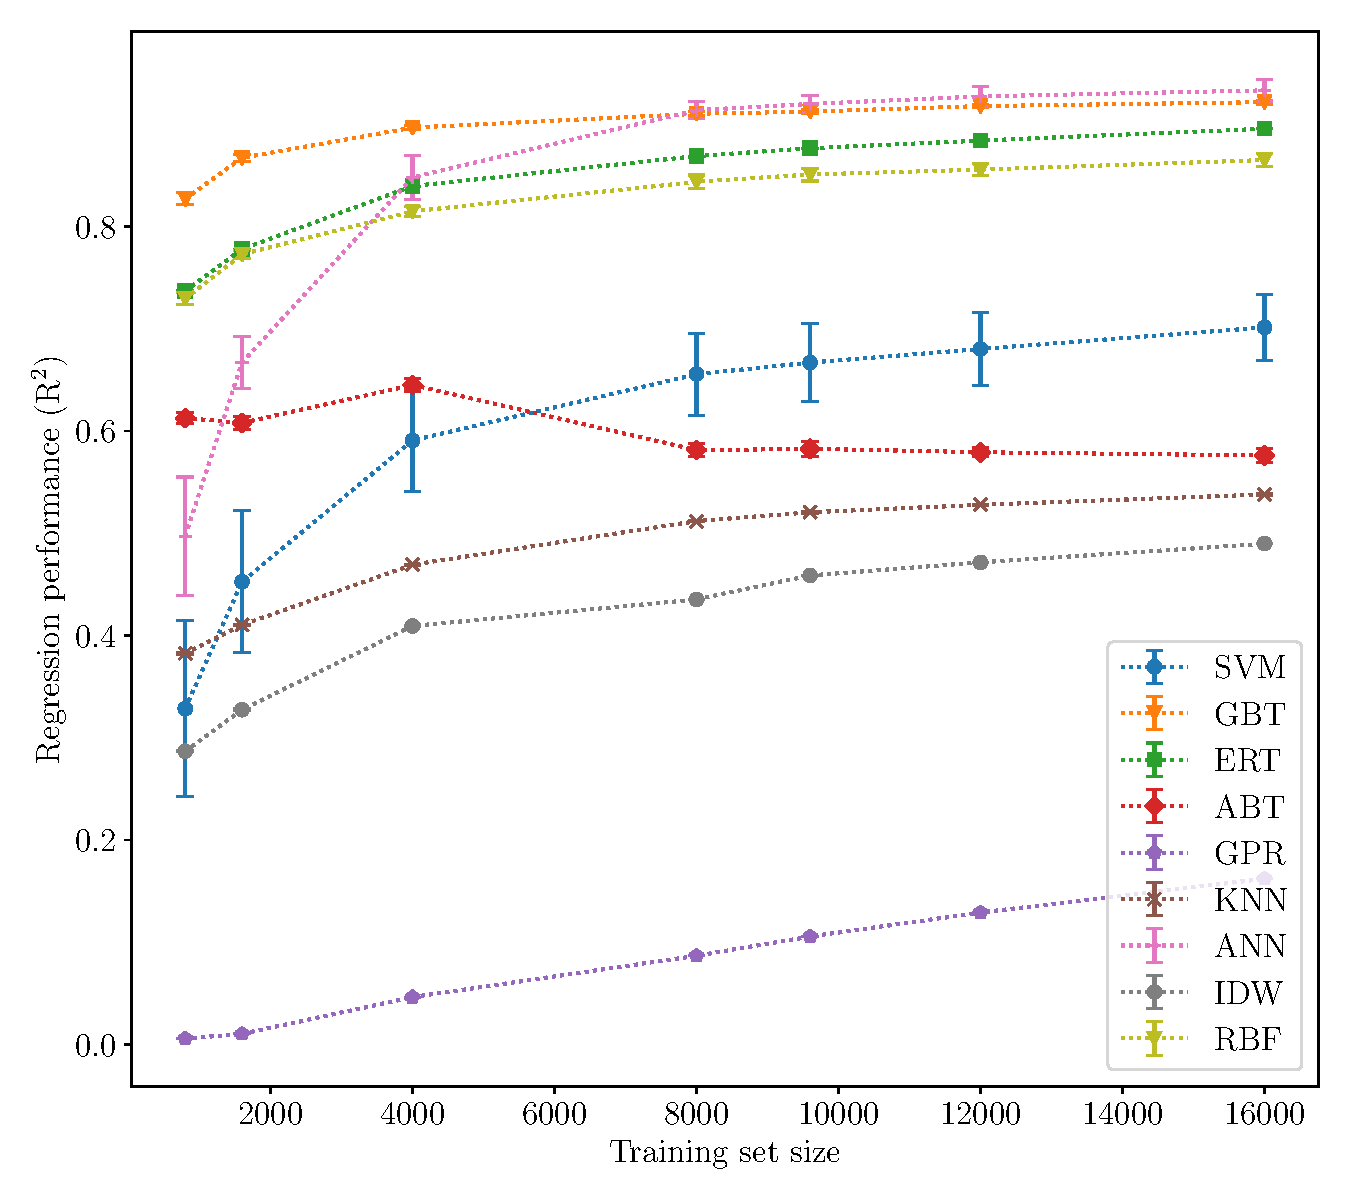
\includegraphics[width=\linewidth]{scaling_metric_r2}
		% TODO: only a placeholder, regenerate when data becomes available
		\caption{Regression performance (as $R^2$)}
	\end{subfigure}\hfill%
	\begin{subfigure}[b]{0.333\textwidth}
		\centering
		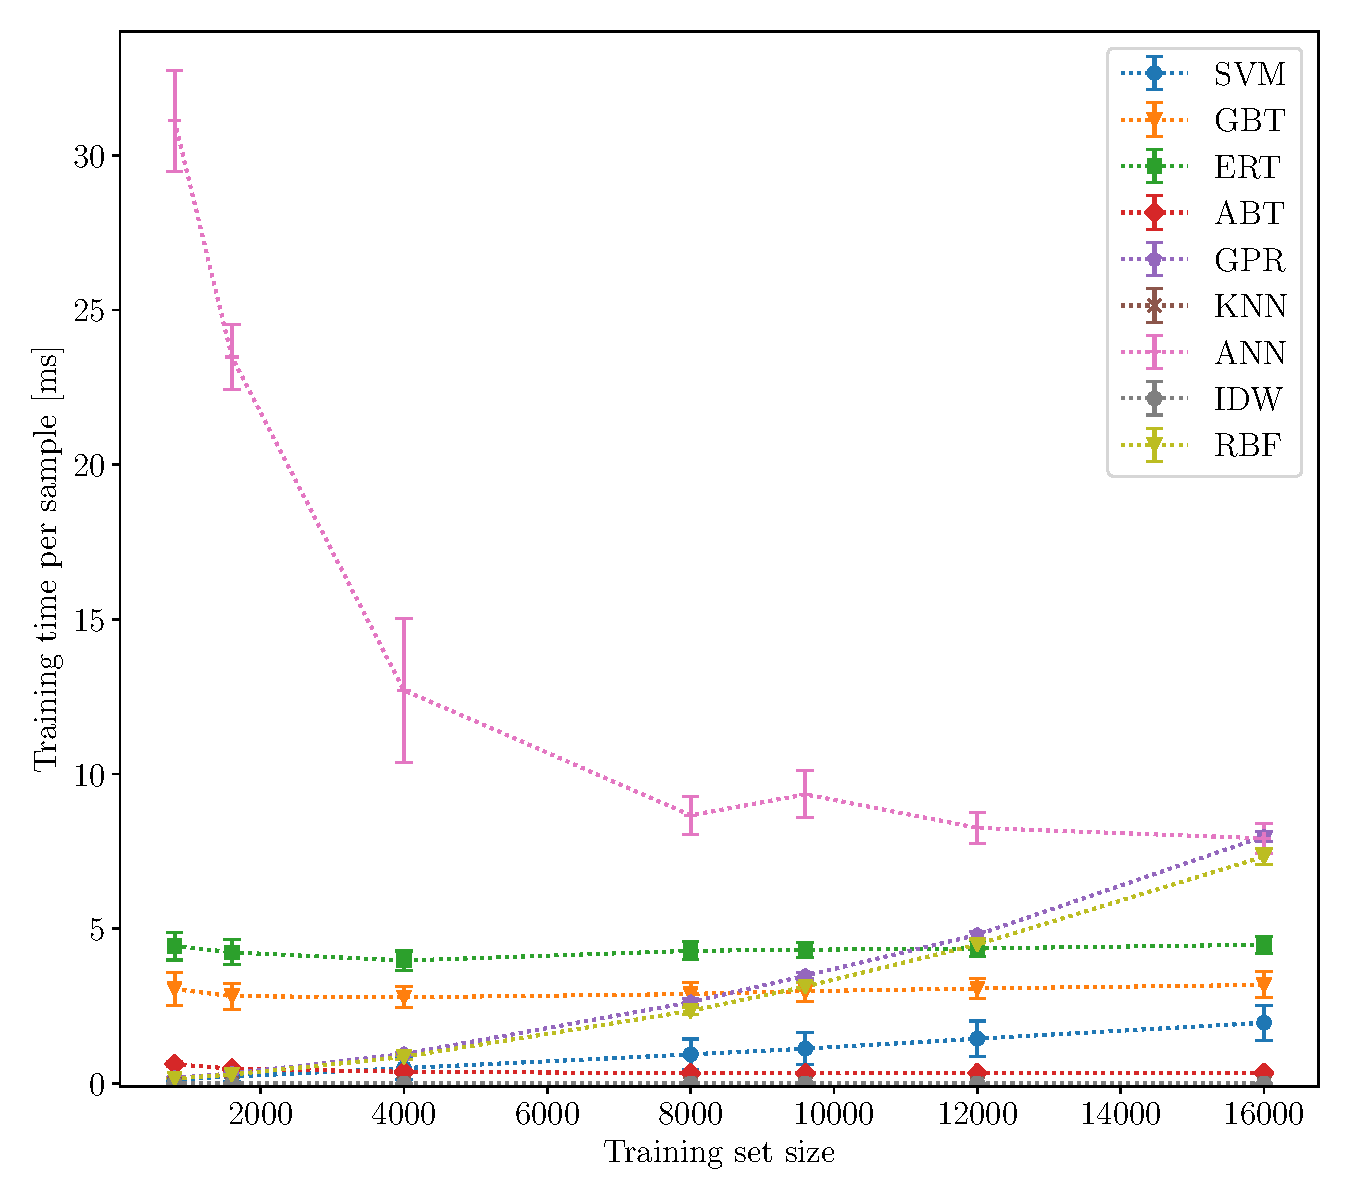
\includegraphics[width=\linewidth]{scaling_time_train}
		% TODO: only a placeholder, regenerate when data becomes available
		\caption{Mean training time}
	\end{subfigure}\hfill%
	\begin{subfigure}[b]{0.333\textwidth}
		\centering
		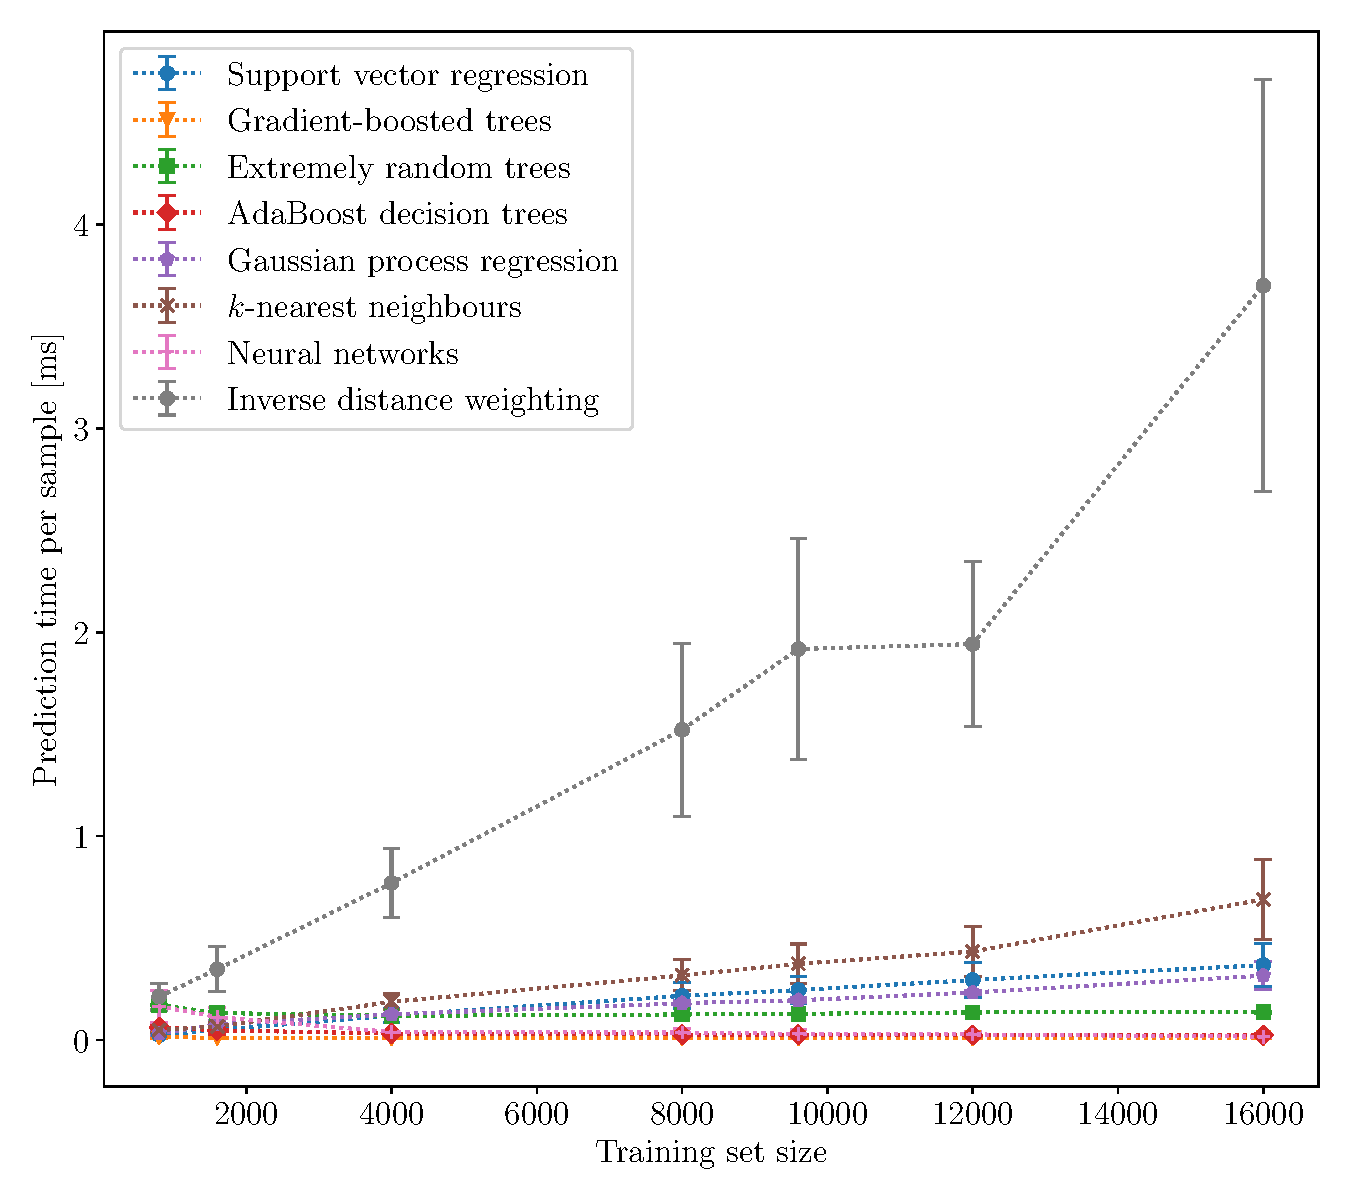
\includegraphics[width=\linewidth]{scaling_time_pred}
		% TODO: only a placeholder, regenerate when data becomes available
		\caption{Mean prediction time}
	\end{subfigure}
	\caption{Various metrics collected during experiment 3 (scaling
	benchmark) displayed as a function of training set size.}
	\label{fig:scaling}
\end{figure}

\subsubsection{Competitive Training}

TODO

\begin{figure}[h]
	\centering
	\begin{subfigure}[b]{0.333\textwidth}
		\centering
		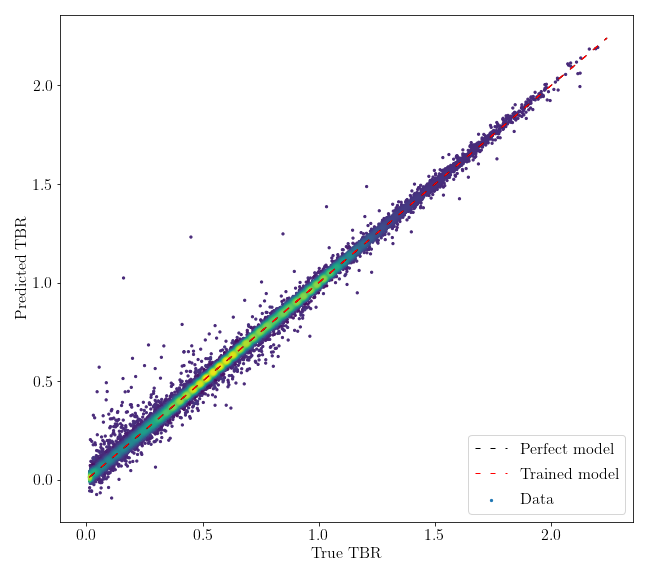
\includegraphics[width=\linewidth]{run1_5ke_1h3f128_4974_performance}
		% TODO: only a placeholder, regenerate when data becomes available
		\caption{Model 1}
	\end{subfigure}\hfill%
	\begin{subfigure}[b]{0.333\textwidth}
		\centering
		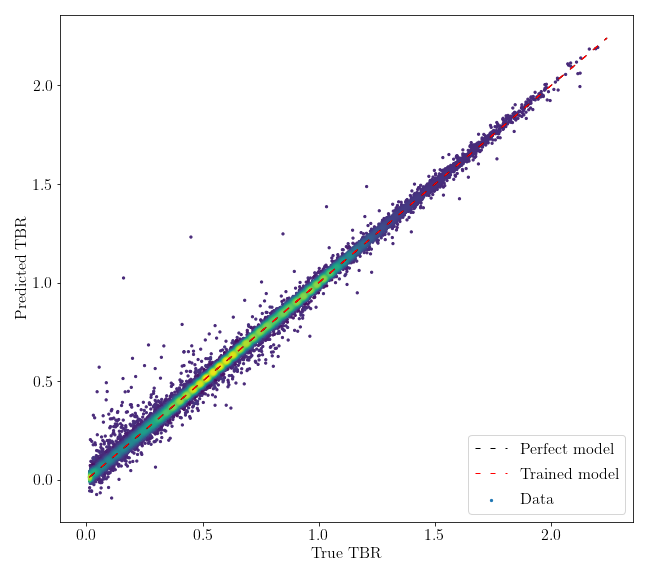
\includegraphics[width=\linewidth]{run1_5ke_1h3f128_4974_performance}
		% TODO: only a placeholder, regenerate when data becomes available
		\caption{Model 2}
	\end{subfigure}\hfill%
	\begin{subfigure}[b]{0.333\textwidth}
		\centering
		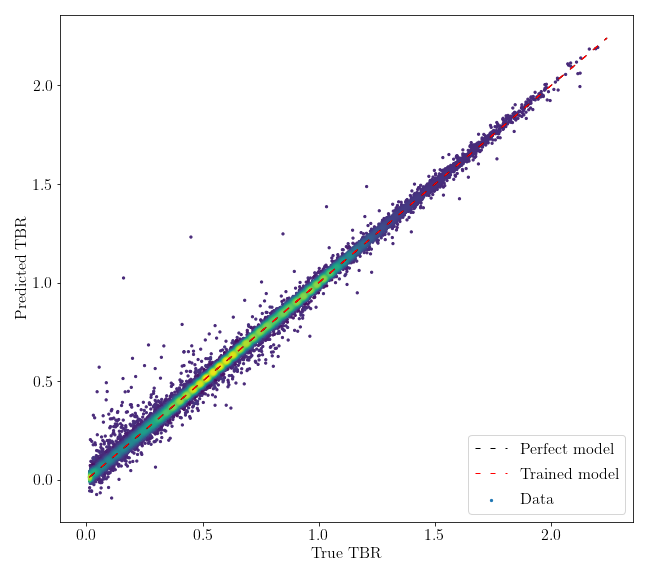
\includegraphics[width=\linewidth]{run1_5ke_1h3f128_4974_performance}
		% TODO: only a placeholder, regenerate when data becomes available
		\caption{Model 3}
	\end{subfigure}

	\vspace{0.75ex}

	\begin{subfigure}[b]{0.333\textwidth}
		\centering
		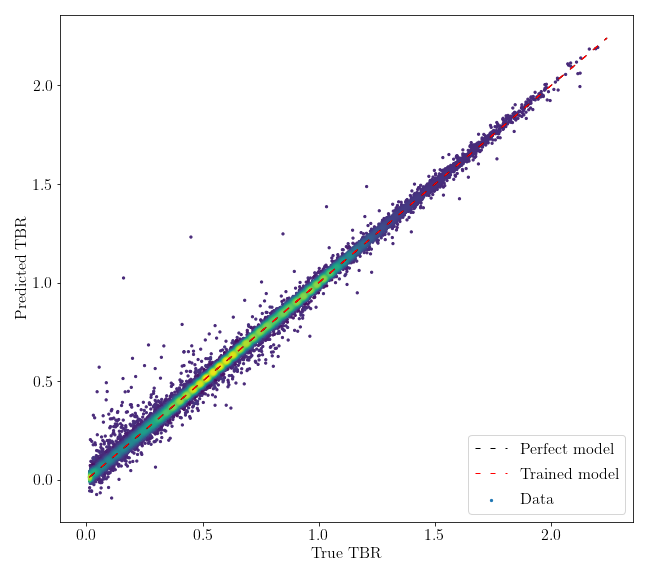
\includegraphics[width=\linewidth]{run1_5ke_1h3f128_4974_performance}
		% TODO: only a placeholder, regenerate when data becomes available
		\caption{Model 1}
	\end{subfigure}\hfill%
	\begin{subfigure}[b]{0.333\textwidth}
		\centering
		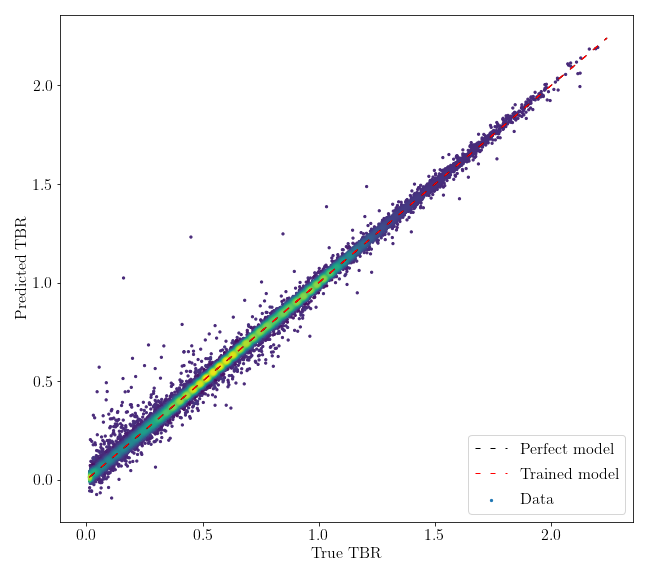
\includegraphics[width=\linewidth]{run1_5ke_1h3f128_4974_performance}
		% TODO: only a placeholder, regenerate when data becomes available
		\caption{Model 2}
	\end{subfigure}\hfill%
	\begin{subfigure}[b]{0.333\textwidth}
		\centering
		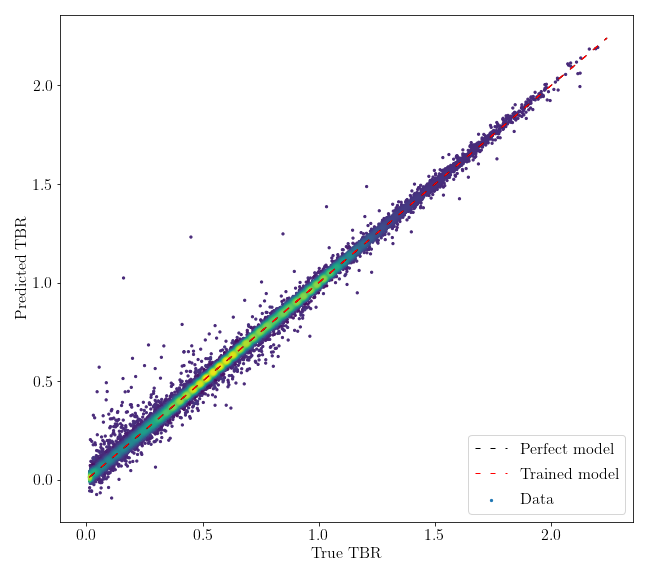
\includegraphics[width=\linewidth]{run1_5ke_1h3f128_4974_performance}
		% TODO: only a placeholder, regenerate when data becomes available
		\caption{Model 3}
	\end{subfigure}
	\caption{Regression performance of the best models trained in experiment~4.}
	\label{fig:reg-performance}
\end{figure}

\subsection{Results of Adaptive Sampling}
\label{sec:adaptiveres}

Define sinusoidal toy model and justify

Explain hyperparameter tests: initsamples, stepsamples, MCMC length

\begin{figure}[h]
    \centering
    \begin{subfigure}[t]{0.5\textwidth}
        \centering
        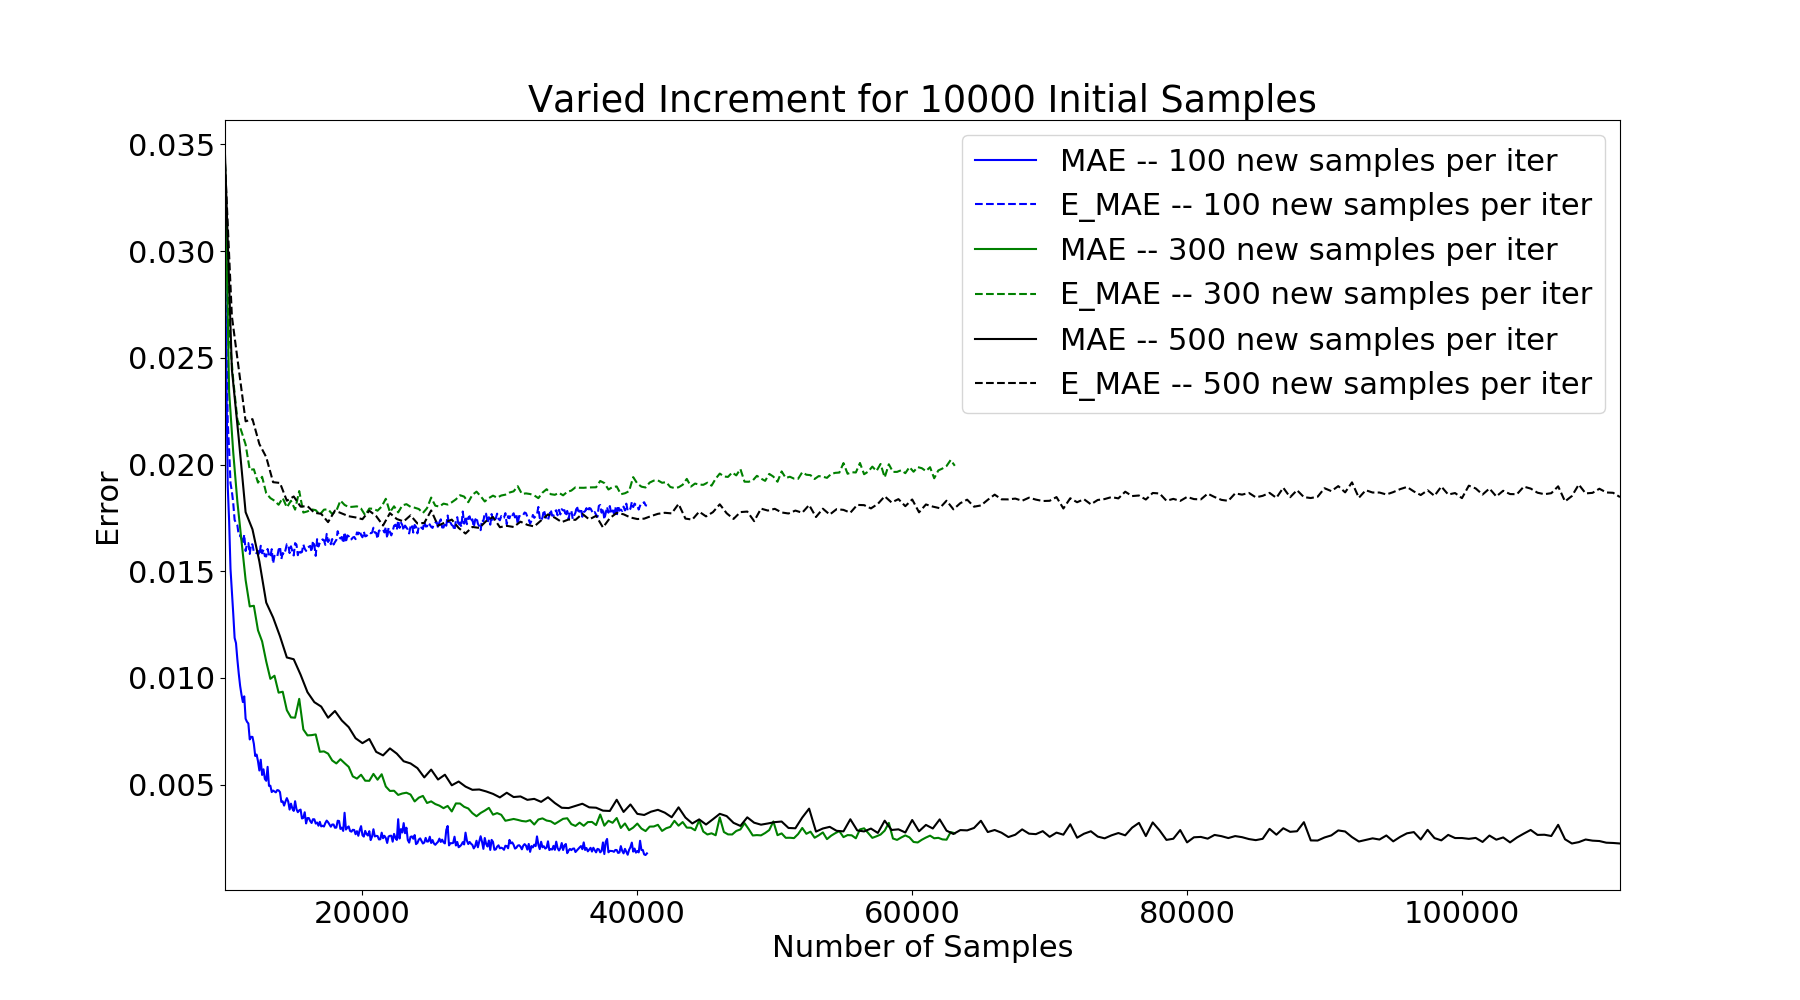
\includegraphics[width=1.1\linewidth]{fig5_qassincrsamp.png}
        \caption{QASS absolute training error over total sample quantity}
    \end{subfigure}%
    ~ 
    \begin{subfigure}[t]{0.5\textwidth}
        \centering
        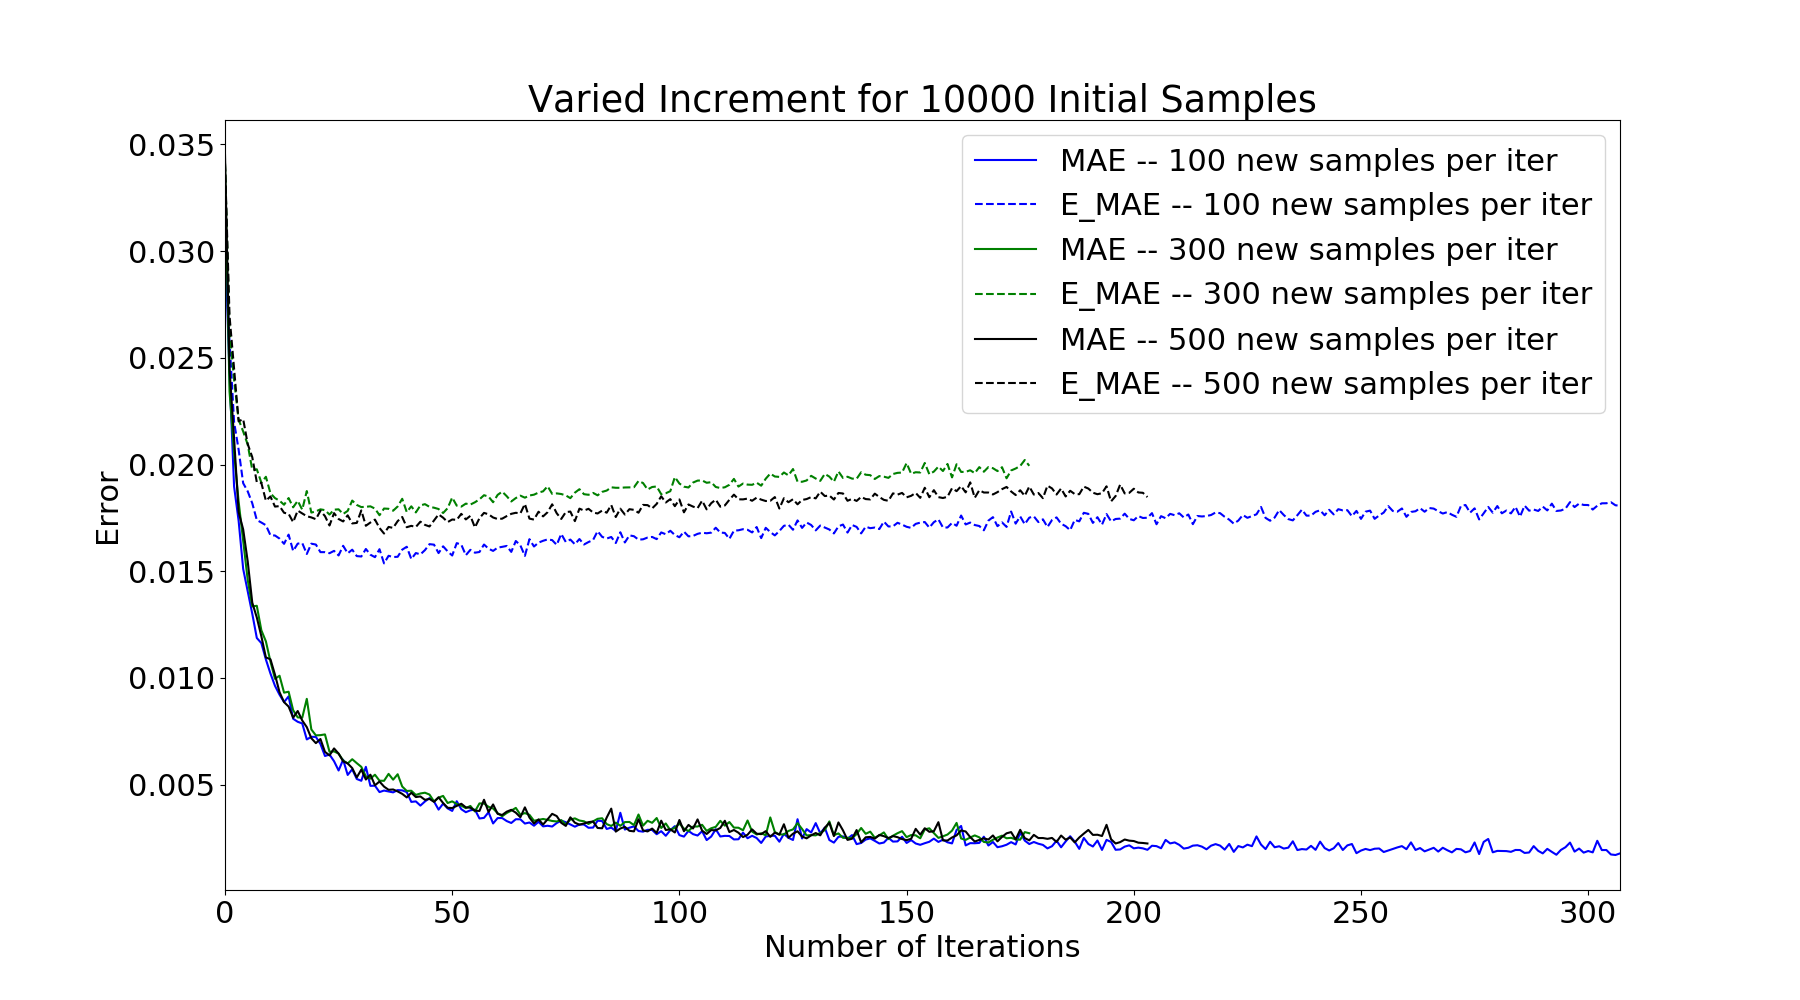
\includegraphics[width=1.1\linewidth]{fig6_qassincrtime.png}
        \caption{QASS absolute training error over number of iterations}
    \end{subfigure}
    \caption{Caption place holder}
\end{figure}

\begin{figure}[h]
  \centering
    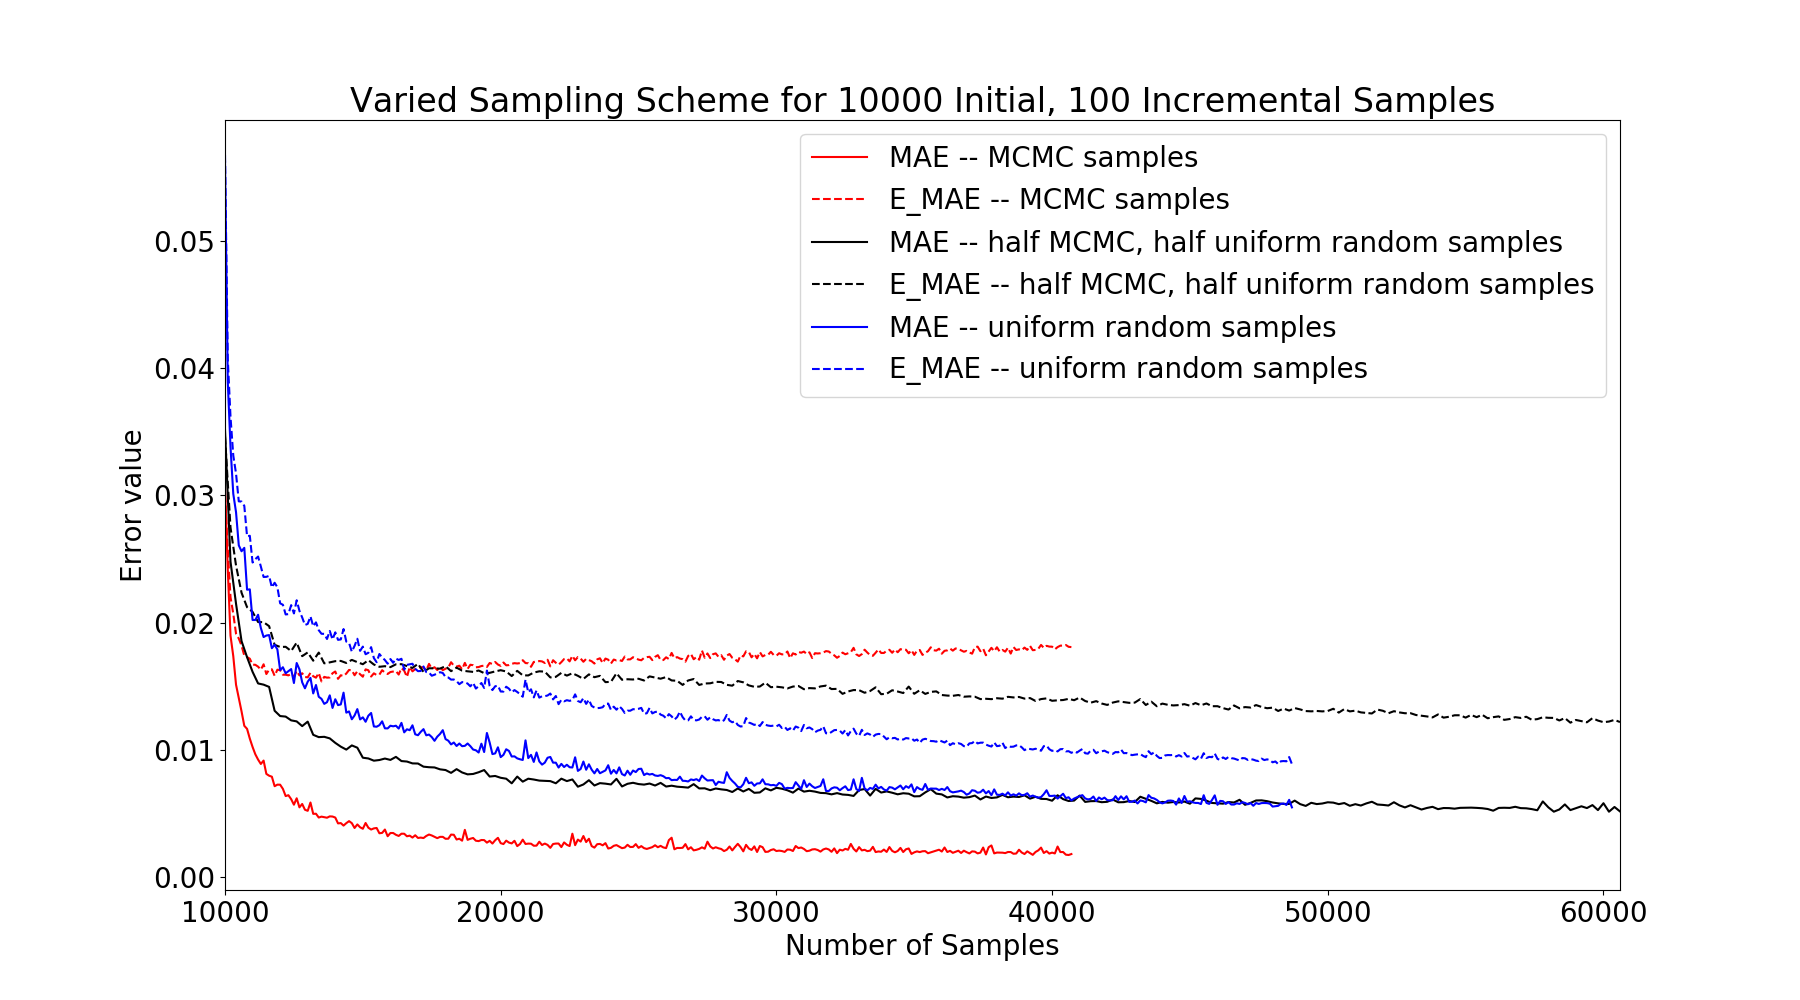
\includegraphics[width=0.8\linewidth]{fig7_qasssampling.png}
    \caption{Absolute training error for QASS, uniform random scheme, and mixed scheme}
  \label{fig:pca}
\end{figure}
